\documentclass[xcolor={x11names,svgnames},x11names,svgnames]{beamer}

%\includeonlyframes{2d}

%\usepackage[]{babel}
\usepackage[T1]{fontenc}
\usepackage{cellspace}

\usepackage{amsmath}
\usepackage{amsfonts}
\usepackage{tikz}
\usepackage{xspace}
\usepackage[normalem]{ulem}
\usepackage{minted}
%\usepackage{fancybox}

%\usepackage{eurosym}
%\usepackage{marvosym}
%\usepackage{pifont}
\usepackage{xcolor}

\newcommand{\bigO}[1]{\ensuremath{\mathcal{O}\left( #1 \right)} }

\DeclareMathOperator*{\argmax}{arg\,max}

\newcommand{\red}{\alert}
\newcommand{\green}{\color{LimeGreen}}
\newcommand{\blue}{\color{cyan}}

\usetikzlibrary{patterns}
%\usetikzlibrary{snakes}
%\usetikzlibrary{arrows}
%\usetikzlibrary{backgrounds}
%\usetikzlibrary{shapes}
%\usetikzlibrary{shadows}
\usetikzlibrary{calc}
\usetikzlibrary{decorations}
\usetikzlibrary{decorations.pathreplacing}
%\usetikzlibrary{decorations.shapes}
%\usetikzlibrary{decorations.markings}
%\usetikzlibrary{positioning}

\definecolor{amethyst}{rgb}{0.6, 0.4, 0.8}
\definecolor{cyan}{rgb}{0,0.6796875,1}

\usecolortheme{rose}
\setbeamertemplate{footline}{}
\setbeamertemplate{navigation symbols}{}

\usepackage{fontspec}
\setsansfont{PalatinoSansLTPro}[
   Path = /home/charles/charles_work/fonts/PalatinoSans/, 
   Extension      = .otf,
   UprightFont    = *-Regular,
   BoldFont= *-Bold ,
   ItalicFont = *-Italic,
   BoldItalicFont = *-BoldIta
]

\author[C.~Bouillaguet]{Charles Bouillaguet \newline
  {\small (\texttt{charles.bouillaguet@lip6.fr})}}

\title{Cours 4 : Algèbre linéaire distribuée}
\date{2021-02-12}

\begin{document}

\begin{frame}[label=title]
  \titlepage
\end{frame}

%%%%%%%%%%%%%%%%%%%%%%%%%%%%%%%%%%%%%%%%%%%%%%%%%%%%%%

\begin{frame}
  \frametitle{Importance of Linear Algebra}

  \begin{alertblock}{Reason}
  Systems of \textbf{linear} equations are the only ones we can solve
    \begin{itemize}
    \item (efficiently, at least)
    \end{itemize}
  \end{alertblock}

  \begin{itemize}
  \item $Ax = b$
  \item $AX = B$  \hfill (multiple right-hand sides)
  \item $\min_x \| Ax - b \|_2$ \hfill (overdetermined linear least squares)
  \item $\min_x \| x \|_2$ s.t. $Ax = b$ \hfill (underdetermined linear least squares)
  \item $Av = \lambda v$ \hfill (eigenvalues/eigenvectors)

  \end{itemize}

  \medskip

  \begin{center}
    \fbox{Basic building block of nearly all scientific computation}
  \end{center}
\end{frame}

%%%%%%%%%%%%%%%%%%%%%%%%%%%%%%%%%%%%%%%%%%%%%%%%%%%%%%

\section{Dense}

\begin{frame}
  \frametitle{BLAS}

  % how to write fast software?
  % use the right tools
  % small set of vesratile and optimized libraries
  
  \begin{block}{Basic Linear Algebra Subroutines}
    \begin{itemize}
    \item Software libraries developped in the 1980's (Fortran-77...)
    \item \red{Simple} and \red{common} operations
    \item \red{heavily optimized}
      \begin{itemize}
      \item[$\Rightarrow$] you willl never do better
      \end{itemize}
    \end{itemize}
  \end{block}

  \begin{exampleblock}{Common HPC Design Strategy}
    \begin{itemize}
    \item More complex linear algebra use the BLAS
    \item Simplifies development
      \begin{itemize}
      \item Just need to remember the interface
      \end{itemize}
    \item High-speed BLAS $\leadsto$ high-speed software
    \item Ugly low-level optimizations \emph{confined} inside the BLAS
    \end{itemize}
  \end{exampleblock}  
\end{frame}

%%%%%%%%%%%%%%%%%%%%%%%%%%%%%%%%%%%%%%%%%%%%%%%%%%%%%%

\begin{frame}
  \frametitle{BLAS Levels}

  \[
    \texttt{x} \in \{ \texttt{S}, \texttt{D}, \texttt{C}, \texttt{Z} \}
  \]
  
  \begin{block}{Level 1 Routines: \red{vector} operations}
    \begin{itemize}
    \item \texttt{xSCAL} : $x \gets \alpha x$
    \item \texttt{xCOPY} : $x \gets y$
    \item \texttt{xAXPY} : $y \gets \alpha x + y$
    \item \texttt{xDOT} : $\alpha \gets x \cdot y$
    \item \texttt{xNORM} : $\alpha \gets \| x \|_2$
    \item \texttt{xSUM} : $k \gets \sum_i | x_i |$
    \item \texttt{IxAMAX} : $k \gets \argmax_i | x_i |$
    \end{itemize}
  \end{block}
\end{frame}

%%%%%%%%%%%%%%%%%%%%%%%%%%%%%%%%%%%%%%%%%%%%%%%%%%%%%%%%%%%%%%

\begin{frame}
  \frametitle{BLAS Levels}

  \[
    \texttt{x} \in \{ \texttt{S}, \texttt{D}, \texttt{C}, \texttt{Z} \}
  \]
  
  \begin{block}{Level 2 Routines: \red{matrix-vector} operations}
    \begin{itemize}
    \item Matrix-vector product (\texttt{xGEMV}) 
      \begin{itemize}
      \item $y \gets \alpha Ax + \beta y$
      \item Options to multiply by $A^t$ or $A^h$
      \item Special cases: symmetric $A$ (\texttt{xSYMV}), triangular $A$ (\texttt{xTRMV})
      \end{itemize}

      \medskip
      
    \item Triangular solve (\texttt{xTRSV})
      \begin{itemize}
      \item Solve $Lx = b$ or $Ux = b$
      \end{itemize}

      \medskip
      
    \item Rank-1 update (\texttt{xGER})
      \begin{itemize}
      \item $A \gets A + \alpha x y^t$        
      \end{itemize}
    \end{itemize}
  \end{block}
\end{frame}

%%%%%%%%%%%%%%%%%%%%%%%%%%%%%%%%%%%%%%%%%%%%%%%%%%%%%%%%%%%%%%

\begin{frame}
  \frametitle{BLAS Levels}

  \[
    \texttt{x} \in \{ \texttt{S}, \texttt{D}, \texttt{C}, \texttt{Z} \}
  \]
  
  \begin{block}{Level 3 Routines: \red{matrix-matrix} operations}
    \begin{itemize}
    \item Matrix-Matrix product (\texttt{xGEMM}) 
      \begin{itemize}
      \item $C \gets \alpha AB + \beta C$
      \item Options to use $A^t$ or $B^t$
      \item Special cases: symmetric $A,B$ (\texttt{xSYMM}), triangular $A$ (\texttt{xTRMM})
      \end{itemize}

      \medskip
      
    \item Triangular solve (\texttt{xTRSM}) with multiple right-hand sides
      \begin{itemize}
      \item Solve $LX = B$ or $UX = B$
      \end{itemize}

      \medskip
      
    \item Rank-$k$ symmetric update (\texttt{xSYRK})
      \begin{itemize}
      \item $C \gets \alpha AA^t + \beta C$ 
      \item Symmetric $C$
      \end{itemize}
    \end{itemize}
  \end{block}
\end{frame}

%%%%%%%%%%%%%%%%%%%%%%%%%%%%%%%%%%%%%%%%%%%%%%%%%%%%%%%%%%%%%%%%%%%%%%%%%%%%%%%%%%%%%%%%%

\begin{frame}
  \frametitle{Solving actual problems}

  \begin{center}
    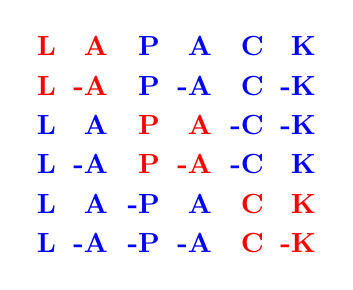
\begin{tikzpicture}[yscale=0.5,xscale=0.66,every node/.style={anchor=south east,font=\bfseries}]
      \node[red] at (0, 5) {L};
      \node[red] at (0, 4) {L};
      \node[blue] at (0, 3) {L};
      \node[blue] at (0, 1) {L};
      \node[blue] at (0, 0) {L};
      \node[blue] at (0, 2) {L};
      
      \node[red] at (1, 5) {A};
      \node[red] at (1, 4) {-A};
      \node[blue]  at (1, 3) {A};
      \node[blue]  at (1, 2) {-A};
      \node[blue] at (1, 1) {A};
      \node[blue] at (1, 0) {-A};

      \node[blue]  at (2, 5) {P};
      \node[blue]  at (2, 4) {P};
      \node[red] at (2, 3) {P};
      \node[red] at (2, 2) {P};
      \node[blue] at (2, 1) {-P};
      \node[blue] at (2, 0) {-P};

      \node[blue]  at (3, 5) {A};
      \node[blue]  at (3, 4) {-A};
      \node[red] at (3, 3) {A};
      \node[red] at (3, 2) {-A};
      \node[blue] at (3, 1) {A};
      \node[blue] at (3, 0) {-A};

      \node[blue] at (4, 5) {C};
      \node[blue] at (4, 4) {C};
      \node[blue] at (4, 3) {-C};
      \node[blue]  at (4, 2) {-C};
      \node[red]  at (4, 1) {C};
      \node[red] at (4, 0) {C};

      \node[blue] at (5, 5) {K};
      \node[blue] at (5, 4) {-K};
      \node[blue] at (5, 3) {-K};
      \node[blue]  at (5, 2) {K};
      \node[red]  at (5, 1) {K};
      \node[red] at (5, 0) {-K};

    \end{tikzpicture}
  \end{center}
  
  \begin{exampleblock}{\textbf{LAPACK}: Linear Algebra PACKage}
    \begin{itemize}
    \item Development started in the 1990's (still active)
    \item Built upon the BLAS
    \item Solve linear systems, least-squares, eigenvalues, etc.
    \item \textbf{Main algorithmic idea}: \red{use level-3 BLAS}
      \begin{itemize}
      \item High \red{arithmetic intensity}
      \item Significant performance gain over naive code
      \end{itemize}
    \end{itemize}
  \end{exampleblock}  
\end{frame}

%%%%%%%%%%%%%%%%%%%%%%%%%%%%%%%%%%%%%%%%%%%%%%%%


  \newcommand{\tikzmat}[2] {
\draw[thick] let \p1 = (#1 |- #2),
                 \p2 = (#2 |- #1) in
   ($ (#1) + (0.05,-0.1) $) -- ++(-0.15, 0)  -- ($ (\p1) + (-0.1,0.1) $) -- ++(0.15,0)
   ($ (\p2) + (-0.05,-0.1) $) -- ++(0.15, 0) -- ($ (#2) + (0.1,0.1) $) -- ++(-0.15,0);
}
  

\begin{frame}
  \frametitle{LU Factorization}

  \begin{center}
    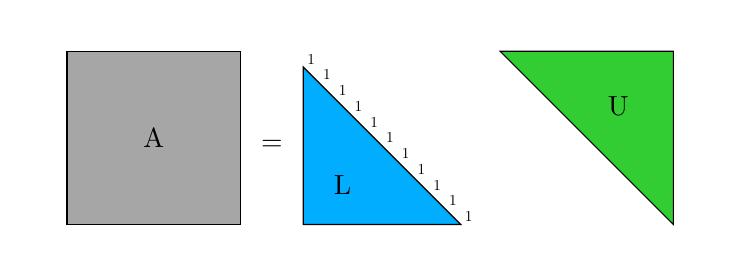
\begin{tikzpicture}
      \useasboundingbox (-0.5,-0.3) rectangle (8.25,2.5);
      
      % L en haut
      \begin{scope}[xshift=3cm]
        \tikzmat{0,0}{2.2,2.2}
        \foreach \i in {0, 0.2, ..., 2}
        \path (\i,2-\i) rectangle node {\scalebox{0.55}{1}} +(0.2,0.2);
        \filldraw[fill=cyan] (0,0) -- ++(0, 2)  -- ++(2,-2) -- cycle;
        \node at (0.5, 0.5) {L};
      \end{scope}
      
      % U en haut
      \begin{scope}[xshift=5.5cm]
        \tikzmat{0,0}{2.2,2.2}
        \draw[fill=LimeGreen] (0,2.2) -- ++(2.2,0) -- ++(0,-2.2) -- cycle;
        \node at (1.5, 1.5) {U};
      \end{scope}
      
      \node at (2.6,1) {$=$};
    
      % matrice grise en haut
      \begin{scope}[xshift=0cm]
        \tikzmat{0,0}{2.2,2.2}
        \filldraw[fill=Gray!70] (0,0) rectangle node{A} +(2.2,2.2);
      \end{scope}
    \end{tikzpicture}
  \end{center}

  \bigskip
  
  Main tool to solve $Ax = b$ when $A$ is invertible

\end{frame}

%%%%

\begin{frame}
  \frametitle{LU Factorization}
%  \framesubtitle{Right-looking Algorithm}

  \begin{columns}
    \begin{column}{5cm}
      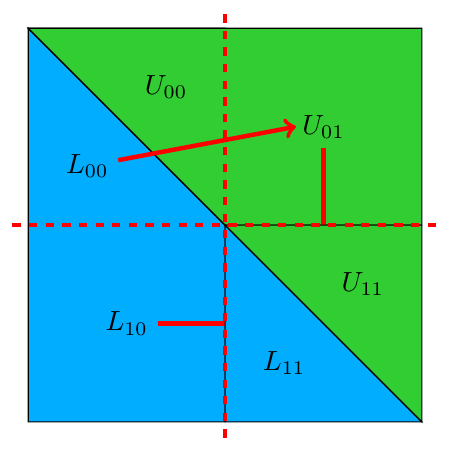
\begin{tikzpicture}
        \draw[red,dotted,use as bounding box] (0, 0) rectangle (5, 5);
    \tikzmat{0,0}{5,5}
    \filldraw[fill=Gray!70] (0, 0) rectangle (5,5);

    \node<1> at (2.5, 2.5) {$A$};

    \node<2> at (1.25, 3.75) {$A_{00}$};
    \node<2> at (1.25, 1.25) {$A_{10}$};

    \node<2-6> at (3.75, 1.25) (a11) {$A_{11}$};
    \node<8> at (3.75, 1.25) (b) {$A_{11} - L_{10} U_{01}$};

    \node<2-4> at (3.75, 3.75) {$A_{01}$};

    \draw<3>[pattern=north west lines] (0,0) rectangle +(2.5, 5);
    \draw<5>[pattern=north west lines] (2.5, 2.5) rectangle +(2.5, 2.5);
    \draw<7,9>[pattern=north west lines] (2.5 , 0) rectangle +(2.5, 2.5);
    
    \filldraw<4->[fill=cyan] (0,5) -- ++(2.5, -2.5) -- (2.5, 0) -- (0, 0) -- cycle;
    \filldraw<4-5>[fill=LimeGreen] (0,5) -- (2.5, 2.5) -- (2.5, 5) -- cycle;
    \filldraw<6->[fill=LimeGreen] (0,5) -- ++(5, 0) -- (5, 2.5) -- (2.5, 2.5) -- cycle;
    
    \node<4-> at (1.25, 1.25) (l10) {$L_{10}$};
    \node<4-> at (0.75, 3.25) (l00) {$L_{00}$};
    \node<4-> at (1.75, 4.25) {$U_{00}$};
    \node<6-> at (3.75, 3.75) (u01) {$U_{01}$};

    \draw<5>[red,ultra thick, ->] (l00) edge (3.4, 3.75);    
    \draw<7>[red,ultra thick, ->] (u01) edge (a11);    
    \draw<7>[red,ultra thick, ->] (l10) edge (a11);    

    
    \filldraw<10>[fill=cyan] (2.5, 2.5) -- (5, 0) -- (2.5, 0) -- cycle;
    \filldraw<10>[fill=LimeGreen] (2.5, 2.5) -- (5, 2.5) -- (5, 0) -- cycle;
    \node<10> at (3.25, 0.75) {$L_{11}$};
    \node<10> at (4.25, 1.75) {$U_{11}$};


      \draw<2->[red, ultra thick, dashed] (-0.2, 2.5) -- (5.2, 2.5);
      \draw<2->[red, ultra thick, dashed] (2.5, -0.2) -- (2.5, 5.2);
  \end{tikzpicture}
\end{column}
\begin{column}{5.5cm}

 \begin{block}{Recursive algorithm}
   \begin{enumerate}
   \item<3-> Factorize left half
   \item<5-> Solve $L_{00} U_{01} = A_{01}$
     \begin{itemize}
     \item level-3 \texttt{TRSM}
     \end{itemize}
     
   \item<7-> $A_{11} \gets A_{11} - L_{10} U_{01}$
     \begin{itemize}
     \item level-3 \texttt{GEMM}
     \end{itemize}
   \item<9-> Factorize $A_{11} - L_{10} U_{01}$
     
   \end{enumerate}
 \end{block}

\end{column}
\end{columns}

\medskip

\[
  \begin{pmatrix}
       A_{00} & A_{01} \\
       A_{10} & A_{11} 
     \end{pmatrix}
     =
     \begin{pmatrix}
       L_{00} &  \\
       L_{10} & L_{11} 
     \end{pmatrix}
     \begin{pmatrix}
       U_{00} & U_{01} \\
       & U_{11} 
     \end{pmatrix}
   \]

   \vspace{-0.5cm}
   
   \begin{align*}     
     L_{00} U_{01} &= A_{01} \\
     L_{11} U_{11} &= A_{11} - L_{10} U_{01}
   \end{align*}
\end{frame}


%%%%%%%%%%%%%%%%%%%%%%%%%%%%%%%%%%%%%%%%%%%%%%%%%%%%%%%%%%%%%%%%%%%%%%%

\begin{frame}
  \frametitle{Distributed LU Factorization}

  \begin{columns}
    \begin{column}{5cm}
  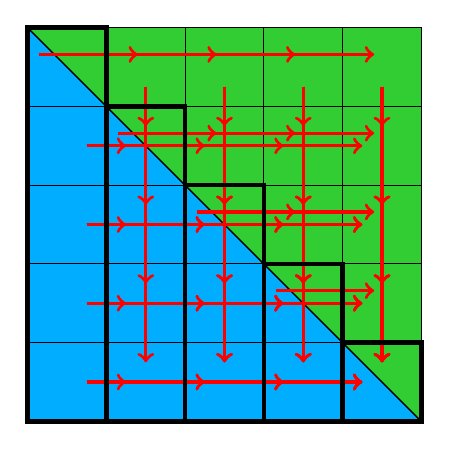
\begin{tikzpicture}
    \path[red,dotted,use as bounding box] (0, 0) rectangle (5, 5);
    \tikzmat{0,0}{5,5}
    \filldraw[fill=Gray!70] (0, 0) rectangle (5,5);

    % 2nd column gets ready
    \draw<7->[pattern=north west lines] (1, 3) rectangle +(1, 1);
    \draw<9->[pattern=north west lines] (1, 2) rectangle +(1, 1);
    \draw<9->[pattern=north west lines] (2, 3) rectangle +(1, 1);

    \draw<9->[pattern=north west lines] (2, 3) rectangle +(1, 1);
    \draw<11->[pattern=north west lines] (1, 1) rectangle +(1, 1);
    \draw<11->[pattern=north west lines] (2, 2) rectangle +(1, 1);
    \draw<11->[pattern=north west lines] (3, 3) rectangle +(1, 1);
    \draw<11->[pattern=north west lines] (3, 3) rectangle +(1, 1);

    \draw<13->[pattern=north west lines] (4, 3) rectangle +(1, 1);
    \draw<13->[pattern=north west lines] (3, 2) rectangle +(1, 1);
    \draw<13->[pattern=north west lines] (2, 1) rectangle +(1, 1);
    \draw<13->[pattern=north west lines] (1, 0) rectangle +(1, 1);

    \draw<15->[pattern=north west lines] (2, 0) rectangle +(1, 1);
    \draw<15->[pattern=north west lines] (3, 1) rectangle +(1, 1);
    \draw<15->[pattern=north west lines] (4, 2) rectangle +(1, 1);

    \draw<17->[pattern=north west lines] (3, 0) rectangle +(1, 1);
    \draw<17->[pattern=north west lines] (4, 1) rectangle +(1, 1);

    \draw<19->[pattern=north west lines] (4, 0) rectangle +(1, 1);

    % 2nd wave
    \draw<19->[pattern=north east lines] (2, 2) rectangle +(1, 1);

    \draw<21->[pattern=north east lines] (3, 2) rectangle +(1, 1);
    \draw<21->[pattern=north east lines] (2, 1) rectangle +(1, 1);

    \draw<23->[pattern=north east lines] (2, 0) rectangle +(1, 1);
    \draw<23->[pattern=north east lines] (3, 1) rectangle +(1, 1);
    \draw<23->[pattern=north east lines] (4, 2) rectangle +(1, 1);

    \draw<25->[pattern=north east lines] (3, 0) rectangle +(1, 1);
    \draw<25->[pattern=north east lines] (4, 1) rectangle +(1, 1);
    
    \draw<27->[pattern=north east lines] (4, 0) rectangle +(1, 1);

    % 3rd wave
    \filldraw<29->[fill=Gray!70]  (3, 1) rectangle +(1, 1);
    \draw<29->[pattern=fivepointed stars]  (3, 1) rectangle +(1, 1);

    \filldraw<31->[fill=Gray!70]  (3, 0) rectangle +(1, 1);
    \draw<31->[pattern=fivepointed stars]  (3, 0) rectangle +(1, 1);

    \filldraw<31->[fill=Gray!70]  (4, 1) rectangle +(1, 1);
    \draw<31->[pattern=fivepointed stars]  (4, 1) rectangle +(1, 1);

    \filldraw<33->[fill=Gray!70]  (4, 0) rectangle +(1, 1);
    \draw<33->[pattern=fivepointed stars]  (4, 0) rectangle +(1, 1);
    
    \filldraw<3->[fill=cyan] (0,5) -- (0, 0) -- (1, 0) -- (1, 4) -- cycle;
    \filldraw<3->[fill=LimeGreen] (0,5) -- ++(1, 0) -- ++(0, -1) -- cycle;
    
    % 4rd wave
    \filldraw<37->[fill=Gray!70]  (4, 0) rectangle +(1, 1);
    \draw<37->[pattern=bricks]  (4, 0) rectangle +(1, 1);


    % U_01
    \filldraw<5->[fill=LimeGreen] (1,5) rectangle ++(1, -1);
    \filldraw<7->[fill=LimeGreen] (2,5) rectangle ++(1, -1);
    \filldraw<9->[fill=LimeGreen] (3,5) rectangle ++(1, -1);
    \filldraw<11->[fill=LimeGreen] (4,5) rectangle ++(1, -1);

        % U_11
    \filldraw<17->[fill=LimeGreen] (2,4) rectangle ++(1, -1);
    \filldraw<19->[fill=LimeGreen] (3,4) rectangle ++(1, -1);
    \filldraw<21->[fill=LimeGreen] (4,4) rectangle ++(1, -1);

    % U_22
    \filldraw<27->[fill=LimeGreen] (3,3) rectangle ++(1, -1);
    \filldraw<29->[fill=LimeGreen] (4,3) rectangle ++(1, -1);

    % U_33
    \filldraw<35->[fill=LimeGreen] (4,2) rectangle ++(1, -1);

    \filldraw<39>[fill=cyan] (4,1) -- (5, 0) -- (4, 0) -- cycle;
    \filldraw<39>[fill=LimeGreen] (4,1) -- ++(1, 0) -- ++(0, -1) -- cycle;
        
    % Attack 2nd col
    \filldraw<15->[fill=cyan] (1,4) -- (1, 0) -- (2, 0) -- (2, 3) -- cycle;
    \filldraw<15->[fill=LimeGreen] (1,4) -- ++(1, 0) -- ++(0, -1) -- cycle;

    % Attack 3rd col
    \filldraw<25->[fill=cyan] (2,3) -- (2, 0) -- (3, 0) -- (3, 2) -- cycle;
    \filldraw<25->[fill=LimeGreen] (2,3) -- ++(1, 0) -- ++(0, -1) -- cycle;

    % Attack 4th col
    \filldraw<33->[fill=cyan] (3,2) -- (3, 0) -- (4, 0) -- (4, 1) -- cycle;
    \filldraw<33->[fill=LimeGreen] (3,2) -- ++(1, 0) -- ++(0, -1) -- cycle;

    
    % grid
    \foreach \i in {1,2,3,4}  {
      \draw[] (\i, 0) -- (\i, 5);
      \draw[] (0, \i) -- (5, \i);
    }

    % L00 propagates to the right
    \draw<4>[red,->,very thick] (0.15, 4.66) -- ++(1.25, 0);
    \draw<6>[red,->,very thick] (0.15, 4.66) -- ++(2.25, 0);
    \draw<8>[red,->,very thick] (0.15, 4.66) -- ++(3.25, 0);
    \draw<10>[red,->,very thick] (0.15, 4.66) -- ++(4.25, 0);

    % L11 propagates to the right
    \draw<16>[red,->,very thick] (1.15, 3.66) -- ++(1.25, 0);
    \draw<18>[red,->,very thick] (1.15, 3.66) -- ++(2.25, 0);
    \draw<20>[red,->,very thick] (1.15, 3.66) -- ++(3.25, 0);
    
    % L22 propagates to the right
    \draw<26>[red,->,very thick] (2.15, 2.66) -- ++(1.25, 0);
    \draw<28>[red,->,very thick] (2.15, 2.66) -- ++(2.25, 0);

    % L33 propagates to the right
    \draw<34>[red,->,very thick] (3.15, 1.66) -- ++(1.25, 0);
    

    
    % first row of U goes down
    \draw<6>[red,->,very thick] (1.5, 4.25) -- ++(0, -0.5);
    \draw<8>[red,->,very thick] (1.5, 4.25) -- ++(0, -1.5);
    \draw<10>[red,->,very thick] (1.5, 4.25) -- ++(0, -2.5);
    \draw<12>[red,->,very thick] (1.5, 4.25) -- ++(0, -3.5);

    \draw<8>[red,->,very thick] (2.5, 4.25) -- ++(0, -0.5);
    \draw<10>[red,->,very thick] (2.5, 4.25) -- ++(0, -1.5);
    \draw<12>[red,->,very thick] (2.5, 4.25) -- ++(0, -2.5);
    \draw<14>[red,->,very thick] (2.5, 4.25) -- ++(0, -3.5);

    \draw<10>[red,->,very thick] (3.5, 4.25) -- ++(0, -0.5);
    \draw<12>[red,->,very thick] (3.5, 4.25) -- ++(0, -1.5);
    \draw<14>[red,->,very thick] (3.5, 4.25) -- ++(0, -2.5);
    \draw<16>[red,->,very thick] (3.5, 4.25) -- ++(0, -3.5);

    \draw<12>[red,->,very thick] (4.5, 4.25) -- ++(0, -0.5);
    \draw<14>[red,->,very thick] (4.5, 4.25) -- ++(0, -1.5);
    \draw<16>[red,->,very thick] (4.5, 4.25) -- ++(0, -2.5);
    \draw<18>[red,->,very thick] (4.5, 4.25) -- ++(0, -3.5);

    % L_01 goes right
    \draw<6>[red,->,very thick] (0.75, 3.5) -- ++(0.5, 0);
    \draw<8>[red,->,very thick] (0.75, 3.5) -- ++(1.5, 0);
    \draw<10>[red,->,very thick] (0.75, 3.5) -- ++(2.5, 0);
    \draw<12>[red,->,very thick] (0.75, 3.5) -- ++(3.5, 0);
    
    \draw<8>[red,->,very thick] (0.75, 2.5) -- ++(0.5, 0);
    \draw<10>[red,->,very thick] (0.75, 2.5) -- ++(1.5, 0);
    \draw<12>[red,->,very thick] (0.75, 2.5) -- ++(2.5, 0);
    \draw<14>[red,->,very thick] (0.75, 2.5) -- ++(3.5, 0);

    \draw<10>[red,->,very thick] (0.75, 1.5) -- ++(0.5, 0);
    \draw<12>[red,->,very thick] (0.75, 1.5) -- ++(1.5, 0);
    \draw<14>[red,->,very thick] (0.75, 1.5) -- ++(2.5, 0);
    \draw<16>[red,->,very thick] (0.75, 1.5) -- ++(3.5, 0);

    \draw<12>[red,->,very thick] (0.75, 0.5) -- ++(0.5, 0);
    \draw<14>[red,->,very thick] (0.75, 0.5) -- ++(1.5, 0);
    \draw<16>[red,->,very thick] (0.75, 0.5) -- ++(2.5, 0);
    \draw<18>[red,->,very thick] (0.75, 0.5) -- ++(3.5, 0);

    % L_11 goes right
    \draw<18>[red,->,very thick] (1.75, 2.5) -- ++(0.5, 0);
    \draw<20>[red,->,very thick] (1.75, 2.5) -- ++(1.5, 0);
    \draw<22>[red,->,very thick] (1.75, 2.5) -- ++(2.5, 0);

    \draw<20>[red,->,very thick] (1.75, 1.5) -- ++(0.5, 0);
    \draw<22>[red,->,very thick] (1.75, 1.5) -- ++(1.5, 0);
    \draw<24>[red,->,very thick] (1.75, 1.5) -- ++(2.5, 0);

    \draw<22>[red,->,very thick] (1.75, 0.5) -- ++(0.5, 0);
    \draw<24>[red,->,very thick] (1.75, 0.5) -- ++(1.5, 0);
    \draw<26>[red,->,very thick] (1.75, 0.5) -- ++(2.5, 0);

    % L_22 goes right
    \draw<28>[red,->,very thick] (2.75, 1.5) -- ++(0.5, 0);
    \draw<30>[red,->,very thick] (2.75, 1.5) -- ++(1.5, 0);

    \draw<30>[red,->,very thick] (2.75, 0.5) -- ++(0.5, 0);
    \draw<32>[red,->,very thick] (2.75, 0.5) -- ++(1.5, 0);

    % L_33 goes right
    \draw<36>[red,->,very thick] (3.75, 0.5) -- ++(0.5, 0);

    
    % second row of U goes down
    \draw<18>[red,->,very thick] (2.5, 3.25) -- ++(0, -0.5);
    \draw<20>[red,->,very thick] (2.5, 3.25) -- ++(0, -1.5);
    \draw<22>[red,->,very thick] (2.5, 3.25) -- ++(0, -2.5);

    \draw<20>[red,->,very thick] (3.5, 3.25) -- ++(0, -0.5);
    \draw<22>[red,->,very thick] (3.5, 3.25) -- ++(0, -1.5);
    \draw<24>[red,->,very thick] (3.5, 3.25) -- ++(0, -2.5);

    \draw<22>[red,->,very thick] (4.5, 3.25) -- ++(0, -0.5);
    \draw<24>[red,->,very thick] (4.5, 3.25) -- ++(0, -1.5);
    \draw<26>[red,->,very thick] (4.5, 3.25) -- ++(0, -2.5);

    % third row of U goes down
    \draw<28>[red,->,very thick] (3.5, 2.25) -- ++(0, -0.5);
    \draw<30>[red,->,very thick] (3.5, 2.25) -- ++(0, -1.5);

    \draw<30>[red,->,very thick] (4.5, 2.25) -- ++(0, -0.5);
    \draw<32>[red,->,very thick] (4.5, 2.25) -- ++(0, -1.5);

    % fourth row of U goes down
    \draw<36>[red,->,very thick] (4.5, 1.25) -- ++(0, -0.5);

    % do 1st col
    \draw<2>[ultra thick] (0, 0) rectangle +(1, 5);
    \draw<14>[ultra thick] (1, 0) rectangle +(1, 4);
    \draw<24>[ultra thick] (2, 0) rectangle +(1, 3);
    \draw<32>[ultra thick] (3, 0) rectangle +(1, 2);
    \draw<38>[ultra thick] (4, 0) rectangle +(1, 1);
  \end{tikzpicture}
\end{column}

\begin{column}{6cm}
  \begin{block}{Remarks}
    \begin{itemize}
    \item 2D distribution of the matrix
    \item<2-> Proc. on a column cooperate: \red{panel factorization}
    \item<4-> Data flow (\red{pipeline})
    \item<14-> 2nd panel factorization
    \item<19-> 1st row/col now inactive
    \item<27-> 2nd row/col now inactive
    \end{itemize}
  \end{block}
\end{column}
\end{columns}

\begin{exampleblock}<39>{Distributed-memory LU}
  \begin{itemize}
  \item Uses 2D \red{cyclic} block distribution to keep everyone busy
  \item Implented in \texttt{HPL} , \texttt{ScaLAPACK}
  \item Major benchmark of HPC machines (``LINPACK'')
  \end{itemize}
\end{exampleblock}
\end{frame}

%%%%%%%%%%%%%%%%%%%%%%%%%%%%%%%%%%%%%%%%%%%%%%%%%%%%%%%%%%%%%%%%%%%%%%

\section{Méthodes Iterative}

%%%%%%%%%%%%%%%%%%%%%%%%%%%%%%%%%%%%%%%%%%%%

\begin{frame}
  \frametitle{Iterative Methods in Linear Algebra}

  Important family of algorithms
  \begin{itemize}
  \item Solving $Ax = b$ or $Ax = \lambda x$
  \item Conjugate gradient, Lanczos, GMRES, etc.
  \end{itemize}

  \begin{block}{Principle}
    \begin{itemize}
    \item Choose an initial vector $x_0$
    \item Iterate the sequence $x_{i+1} = Ax$
    \item At each iteration, build an approximation of the solution
    \item Stop when the process has converged
      \begin{itemize}
      \item If it ever does...
      \end{itemize}
    \end{itemize}    
  \end{block}

  \begin{exampleblock}{Main point}
    
    \begin{itemize}
    \item Bulk of workload: \red{$y \gets Ax$}
      \begin{itemize}
      \item Matrix-vector product (\texttt{GEMV})
      \item Fast when $A$ is a \alert{\textbf{sparse matrix}}
      \end{itemize}
    \end{itemize}
  \end{exampleblock}  
\end{frame}

%%%%%%%%%%%%%%%%%%%%%%%%%%%%%%%%%%%%%%%%%%%

\begin{frame}
  \frametitle{Sparse Linear Algebra}

  \begin{itemize}
  \item Many physical situations yields \red{sparse} linear systems
  \item E.g. Finite Element Method
    \begin{center}
      \includegraphics[width=5cm]{fem_sample} \\
      {\tiny Image: (c) PyCAE} 
    \end{center}
    
  \item One variable per cell
  \item A single equation \red{only} relates variables of \red{neighboring} cells
  \item $Ax = b$ with \red{sparse} A (mostly zero coefficients)
  \end{itemize}
\end{frame}

%%%%%%%%%%%%%%%%%%%%%%%%%%%%%%%%%%%%%%%%%%%%

\begin{frame}
  \frametitle{Sparse Matrices}

  \begin{block}{Goals when dealing with sparse matrices}
    \begin{itemize}
    \item Don't store 0
    \item Don't compute $0 + x$ and $0 \times x$
    \end{itemize}
  \end{block}
  
  \begin{center}
    \includegraphics[width=3cm]{sparse.png} \\
    {\tiny Image: (c) T. davis} 
  \end{center}
  
  \begin{block}{Most important parameter: \textbf{density}}
    \begin{itemize}
    \item Proportion of \red{non-zero} coefficients
    \item density $< 0.01$ (say) $\leadsto$ sparse
    \end{itemize}
  \end{block}
  
\end{frame}
  

%%%%%%%%%%%%%%%%%%%%%%%%%%%%%%%%%%%%%%%%%%%%

\begin{frame}[fragile]
  \frametitle{Matrix-Vector product (\texttt{GEMV})}
  \framesubtitle{$y \gets y + \alpha Ax$}
  \begin{alertblock}{Dense \texttt{GEMV}}
    \begin{itemize}
    \item All matrix coeffs are contiguous in memory
    \end{itemize}
    \begin{minted}{C}
for (int i = 0; i < n; i++)               // 3nm FLOP
    for (int j = 0; j < m; j++)
        y[i] += alpha * A[i*m + j] * x[j]; 
      \end{minted}
    \end{alertblock}
  
  \begin{exampleblock}{Sparse \texttt{GEMV}}
    \begin{itemize}
      \item Only $\texttt{nz} \lll nm$ non-zero coeffs
      \item Idea: store list of $(i, j, x)$ such that $A_{ij} = x$ (and $x \neq 0)$
        \begin{itemize}
        \item 3 arrays: \texttt{Ai}, \texttt{Aj}, \texttt{Ax}
        \item $k$-th coeff: $(\texttt{Ai[k]}, \texttt{Aj[k]}, \texttt{Ax[k]})$
        \end{itemize}
      \end{itemize}
      \begin{minted}{C}
for (int k = 0; k < nz; k++)              // 3nz FLOP
    y[Ai[k]] += alpha * Ax[k] * x[Aj[k]]; 
    \end{minted}
  \end{exampleblock}
\end{frame}

%%%%%%%%%%%%%%%%%%%%%%%%%%%%%%%%%%%%%%%%%%%% 

\begin{frame}
  \frametitle{Recurring problem in HPC}

  \begin{block}{Iterative methods with sparse matrices}
    \begin{itemize}
    \item compute $x_{i+1} = A x_i$
    \item For $i=1, 2, 3,  4, 5, \dots$
    \item With large, sparse matrix $A$
    \item \red{In parallel}
      \begin{itemize}
      \item Need $x_{i+1}$ to start $x_{i+2}$
      \item Iterations are necessarily \red{Sequential} 
      \item[$\Rightarrow$] Parallelize the \textbf{matrix-vector product}
      \end{itemize}
    \end{itemize}
  \end{block}  
  
  \begin{exampleblock}{Data parallelism}
    \begin{itemize}
    \item $A$ is \textbf{distributed} between processes (how?)
    \item $x_i$ is \textbf{distributed} between processes (how?)
    \item $x_{i+1}$ must be distributed \red{identically} to iterate
    \end{itemize}
  \end{exampleblock}
  
\end{frame}

%%%%%%%%%%%%%%%%%%%%%%%%%%%%%%%%%%%%%%%%%%%

\begin{frame}[label=1d]
  \frametitle{Distributed Matrix-Vector Product}
  \framesubtitle{1D block distribution (per rows)}

  \begin{block}{Data distribution}
    \begin{itemize}
    \item[$M$] : 1D block distribution (blocks of rows)
    \item[$x$] : owned by all processes
    \item[$y$] : owned by all processes
    \end{itemize}
  \end{block}


  \begin{center}
    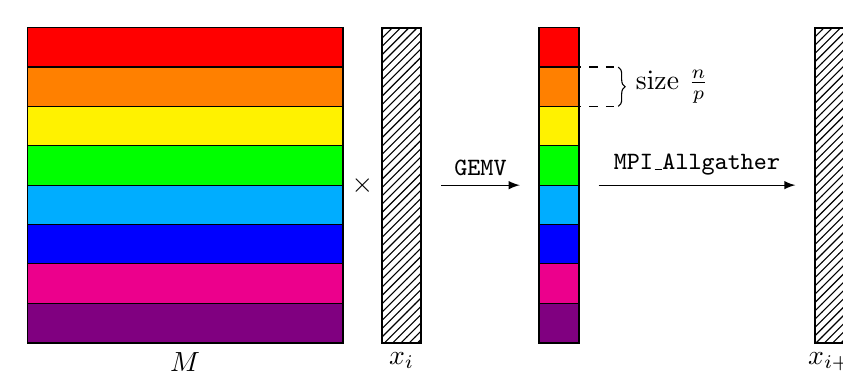
\begin{tikzpicture}[>=latex]
      \path[red,dotted,use as bounding box] (0,0) rectangle (10, 4);
      \draw[<->] (-0.5,0) -- node[left] {$n$} +(0, 4);
  
      % matrix
      \draw[thick] (0,0) rectangle (4,4);
      \filldraw[fill=red]     (0, 3.5) rectangle +(4, 0.5);
      \filldraw[fill=orange]  (0, 3  ) rectangle +(4, 0.5);
      \filldraw[fill=yellow]  (0, 2.5) rectangle +(4, 0.5);
      \filldraw[fill=green]   (0, 2  ) rectangle +(4, 0.5);
      \filldraw[fill=cyan]    (0, 1.5) rectangle +(4, 0.5);
      \filldraw[fill=blue]    (0, 1  ) rectangle +(4, 0.5);
      \filldraw[fill=magenta] (0, 0.5) rectangle +(4, 0.5);
      \filldraw[fill=violet]  (0, 0  ) rectangle +(4, 0.5);
      
      \node[below] at (2,0) {$M$};

      \node at (4.25,2) {$\times$};
      
      \draw[thick,pattern=north east lines] (4.5,0) rectangle +(0.5,4);
      \node[below] at (4.75,0) {$x_i$};
      
      \draw[->] (5.25, 2) -- node[above,font=\small] {\texttt{GEMV}} +(1 ,0);

      \begin{scope}[xshift=0.5cm]
        \draw[thick] (6,0) rectangle +(0.5,4);
        \filldraw[fill=red]     (6, 3.5) rectangle +(0.5, 0.5);
        \filldraw[fill=orange]  (6, 3  ) rectangle +(0.5, 0.5);
        \filldraw[fill=yellow]  (6, 2.5) rectangle +(0.5, 0.5);
        \filldraw[fill=green]   (6, 2  ) rectangle +(0.5, 0.5);
        \filldraw[fill=cyan]    (6, 1.5) rectangle +(0.5, 0.5);
        \filldraw[fill=blue]    (6, 1  ) rectangle +(0.5, 0.5);
        \filldraw[fill=magenta] (6, 0.5) rectangle +(0.5, 0.5);
        \filldraw[fill=violet]  (6, 0  ) rectangle +(0.5, 0.5);
      \end{scope}

    \draw[->] (7.25, 2) -- node[above,font=\small] {\texttt{\texttt{MPI\_Allgather}}} +(2.5, 0);
      
      \draw[dashed] (6.5, 3) -- +(1, 0);
      \draw[dashed] (6.5, 3.5) -- +(1, 0);
      \draw[decorate,decoration={brace,mirror}] (7.5, 3) --  node[right=1mm] {size $\frac{n}{p}$} +(0, 0.5);

      % x_i+1
      \draw[thick,pattern=north east lines] (10,0) rectangle +(0.5,4);
      \node[below] at (10.25,0) {$x_{i+1}$};
    \end{tikzpicture}
  \end{center}
\end{frame}

%%%%%%%%%%%%%%%%%%%%%%%%%%%%%%%%%%%%%%%%%%%

\begin{frame}[label=1d]
%  \frametitle{Distributed Matrix-Vector Product (1D per rows)}

  \begin{alertblock}{Machine parameters}
    \begin{itemize}
    \item $C$ = processor FLOP/s
    \item $D$ = network bandwidth (float / s)
    \end{itemize}
  \end{alertblock}

  \begin{exampleblock}{Matrix characteristics}
    \begin{itemize}
    \item $n$ = size
    \item $d$ = \emph{density} ($dn^2$ non-zero coeffs)
%    \item[$\Rightarrow$] $3 d n^2$ FLOP / iteration
    \end{itemize}
  \end{exampleblock}

  \begin{center}
    \begin{tabular}{|c||c|c|}
      \hline
      & \texttt{GEMV}  & \texttt{MPI\_Allgather} \\
      \hline\hline
      Sequential           & $3 d n^2 / C$ &    0 \\
      \hline
      Distributed          & $3 d n^2 / (pC)$ & $n / D$ \\
      \hline
    \end{tabular}
  \end{center}

  \[
    \mathrm{Speedup} = \frac{d n^2}{C} / (\frac{d n^2}{pC} + \frac{n}{D}) \leq d n \frac{D}{C}
  \]

  \begin{itemize}
  \item $D/C$ = ``machine balance'' = very important
 \end{itemize}
\end{frame}

%%%%%%%%%%%%%%%%%%%%%%%%%%%%%%%%%%%%%%%% 

\begin{frame}[label=1d]
  \frametitle{Communication Limits Acceleration}
  
  \begin{center}
    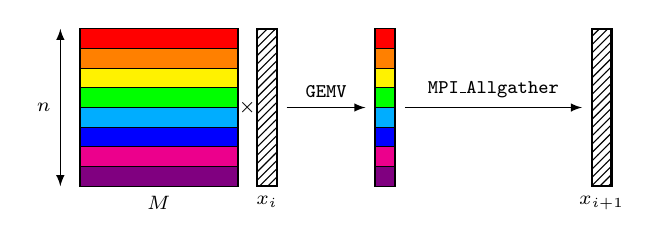
\begin{tikzpicture}[scale=0.5, >=latex, every node/.style={font=\scriptsize}]
      \draw[<->] (-0.5,0) -- node[left] {$n$} +(0, 4);
  
      % matrix
      \draw[thick] (0,0) rectangle (4,4);
      \filldraw[fill=red]     (0, 3.5) rectangle +(4, 0.5);
      \filldraw[fill=orange]  (0, 3  ) rectangle +(4, 0.5);
      \filldraw[fill=yellow]  (0, 2.5) rectangle +(4, 0.5);
      \filldraw[fill=green]   (0, 2  ) rectangle +(4, 0.5);
      \filldraw[fill=cyan]    (0, 1.5) rectangle +(4, 0.5);
      \filldraw[fill=blue]    (0, 1  ) rectangle +(4, 0.5);
      \filldraw[fill=magenta] (0, 0.5) rectangle +(4, 0.5);
      \filldraw[fill=violet]  (0, 0  ) rectangle +(4, 0.5);
      
      \node[below] at (2,0) {$M$};

      \node at (4.25,2) {$\times$};
      
      \draw[thick,pattern=north east lines] (4.5,0) rectangle +(0.5,4);
      \node[below] at (4.75,0) {$x_i$};
      
      \draw[->] (5.25, 2) -- node[above,font=\scriptsize] {\texttt{GEMV}} +(2 ,0);

      \begin{scope}[xshift=7.5cm]
        \draw[thick] (0,0) rectangle +(0.5,4);
        \filldraw[fill=red]     (0, 3.5) rectangle +(0.5, 0.5);
        \filldraw[fill=orange]  (0, 3  ) rectangle +(0.5, 0.5);
        \filldraw[fill=yellow]  (0, 2.5) rectangle +(0.5, 0.5);
        \filldraw[fill=green]   (0, 2  ) rectangle +(0.5, 0.5);
        \filldraw[fill=cyan]    (0, 1.5) rectangle +(0.5, 0.5);
        \filldraw[fill=blue]    (0, 1  ) rectangle +(0.5, 0.5);
        \filldraw[fill=magenta] (0, 0.5) rectangle +(0.5, 0.5);
        \filldraw[fill=violet]  (0, 0  ) rectangle +(0.5, 0.5);
      \end{scope}

    \draw[->] (8.25, 2) -- node[above,font=\scriptsize] {\texttt{MPI\_Allgather}} +(4.5, 0);
      
      % x_i+1
      \draw[thick,pattern=north east lines] (13,0) rectangle +(0.5,4);
      \node[below] at (13.25,0) {$x_{i+1}$};
    \end{tikzpicture}
  \end{center}

\vspace{0.5cm}
  
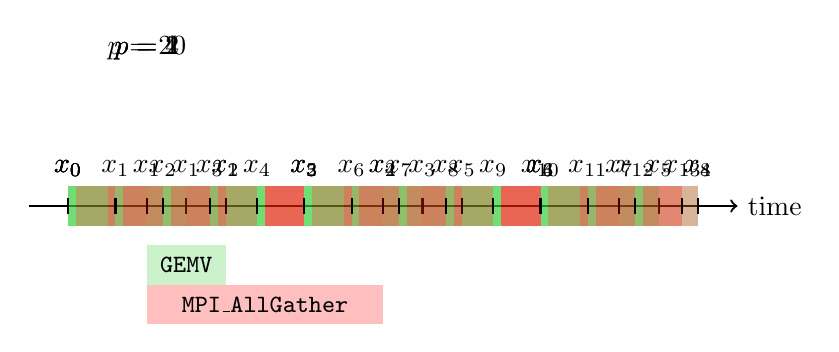
\begin{tikzpicture}
    \node<1> at (1, 2) {$p=1$};
    \node<2> at (1, 2) {$p=2$};
    \node<3> at (1, 2) {$p=4$};
    \node<4> at (1, 2) {$p=20$};
    
    \draw[thick, ->] (-0.5, 0) -- (8.5, 0) node[right] {time};

    
    \foreach \i in {0, 1, 2, 3}  {
      \fill<1>[fill=LimeGreen, nearly transparent] (\i*2cm, -0.25) rectangle +(2, 0.5);
    }
    \foreach \i in {0, 1, 2, 3, 4} {
      \draw<1>[thick] (\i*2cm, -0.1) -- +(0, 0.2);
      \node<1>[anchor=south] at (\i*2cm, 0.25) {$x_\i$};
    }

    % p = 2
    \foreach \i in {0, 1, 2, 3, 4}  {
      \fill<2>[fill=LimeGreen, nearly transparent] (\i*1.5cm, -0.25) rectangle +(1, 0.5);
      \fill<2>[fill=red, nearly transparent] (\i*1.5cm, 0) +(1, -0.25) rectangle +(1.5, 0.25);
    }
    \foreach \i in {0, 1, 2, 3, 4, 5} {
      \draw<2>[thick] (\i*1.5cm, -0.1) -- +(0, 0.2);
      \node<2>[anchor=south] at (\i*1.5cm, 0.25) {$x_\i$};
    }

    % p = 4
    \foreach \i in {0, 1, 2, ..., 7}  {
      \fill<3>[fill=LimeGreen, nearly transparent] (\i*1cm, -0.25) rectangle +(0.5, 0.5);
      \fill<3>[fill=red, nearly transparent] (\i*1cm+0.5cm, -0.25)  rectangle +(0.5, 0.5);
    }
    \foreach \i in {0, 1, ..., 8} {
      \draw<3>[thick] (\i*1cm, -0.1) -- +(0, 0.2);
      \node<3>[anchor=south] at (\i*1cm, 0.25) {$x_\i$};
    }

    % p = 20
    \foreach \i in {0, 1, 2, ..., 12}  {
      \fill<4>[fill=LimeGreen, nearly transparent] (\i*0.6cm, -0.25) rectangle +(0.1, 0.5);
      \fill<4>[fill=red, nearly transparent] (\i*0.6cm+0.1cm, -0.25)  rectangle +(0.5, 0.5);
    }
    \foreach \i in {0, 1, ..., 13} {
      \draw<4>[thick] (\i*0.6cm, -0.1) -- +(0, 0.2);
      \node<4>[anchor=south] at (\i*0.6cm, 0.25) {$x_{\i}$};
    }

    
    \fill[fill=LimeGreen, nearly transparent] (1, -1) rectangle +(1, 0.5);
    \path (1, -1) rectangle node[font=\small] {\texttt{GEMV}} +(1, 0.5);

    \fill[fill=red, nearly transparent] (1, -1.5) rectangle +(3, 0.5);
    \path (1, -1.5) rectangle node[font=\small] {\texttt{MPI\_AllGather}} +(3, 0.5);
  \end{tikzpicture}
\end{frame}


%%%%%%%%%%%%%%%%%%%%%%%%%%%%%%%%%%%%%%%%%%% 

\begin{frame}
  \frametitle{Distributed Matrix-Vector Product}
  \framesubtitle{1D block distribution (per columns)}

  \begin{block}{Data distribution}
    \begin{itemize}
    \item[$M$] : 1D block distribution (blocks of columnss)
    \item[$x$] : 1D block distribution
    \item[$y$] : 1D block distribution
    \end{itemize}
  \end{block}


  \begin{center}
    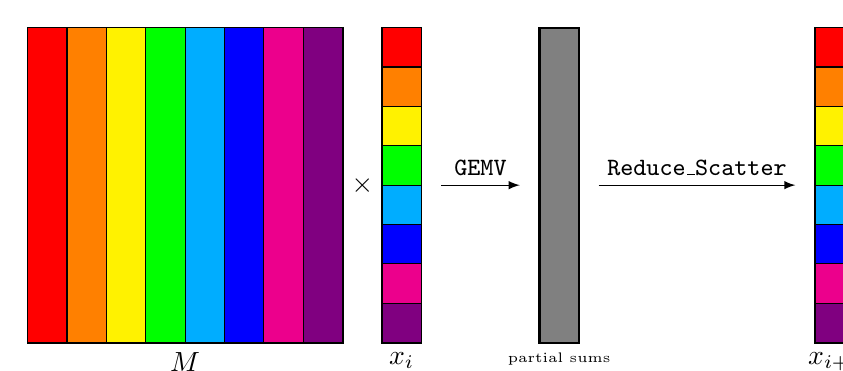
\begin{tikzpicture}[>=latex]
      \path[red,dotted,use as bounding box] (0,0) rectangle (10, 4);
      \draw[<->] (-0.5,0) -- node[left] {$n$} +(0, 4);
  
      % matrix
      \draw[thick] (0,0) rectangle (4,4);
      \filldraw[fill=red]     (0  , 0) rectangle +(0.5, 4);
      \filldraw[fill=orange]  (0.5, 0) rectangle +(0.5, 4);
      \filldraw[fill=yellow]  (1.0, 0) rectangle +(0.5, 4);
      \filldraw[fill=green]   (1.5, 0) rectangle +(0.5, 4);
      \filldraw[fill=cyan]    (2.0, 0) rectangle +(0.5, 4);
      \filldraw[fill=blue]    (2.5, 0) rectangle +(0.5, 4);
      \filldraw[fill=magenta] (3.0, 0) rectangle +(0.5, 4);
      \filldraw[fill=violet]  (3.5, 0) rectangle +(0.5, 4);
      
      \node[below] at (2,0) {$M$};

      \node at (4.25,2) {$\times$};
      
      \begin{scope}[xshift=4.5cm]
        \draw[thick] (0,0) rectangle +(0.5,4);
        \filldraw[fill=red]     (0, 3.5) rectangle +(0.5, 0.5);
        \filldraw[fill=orange]  (0, 3  ) rectangle +(0.5, 0.5);
        \filldraw[fill=yellow]  (0, 2.5) rectangle +(0.5, 0.5);
        \filldraw[fill=green]   (0, 2  ) rectangle +(0.5, 0.5);
        \filldraw[fill=cyan]    (0, 1.5) rectangle +(0.5, 0.5);
        \filldraw[fill=blue]    (0, 1  ) rectangle +(0.5, 0.5);
        \filldraw[fill=magenta] (0, 0.5) rectangle +(0.5, 0.5);
        \filldraw[fill=violet]  (0, 0  ) rectangle +(0.5, 0.5);
      \end{scope}

      \node[below] at (4.75,0) {$x_i$};
      
      \draw[->] (5.25, 2) -- node[above,font=\small] {\texttt{GEMV}} +(1 ,0);

      \draw[thick,fill=gray] (6.5,0) rectangle +(0.5,4);
      \node[below] at (6.75,0) {\tiny partial sums};

      
      \draw[->] (7.25, 2) -- node[above,font=\small] {\texttt{\texttt{Reduce\_Scatter}}} +(2.5, 0);
      
      % x_i+1
      \begin{scope}[xshift=10cm]
        \draw[thick] (0,0) rectangle +(0.5,4);
        \filldraw[fill=red]     (0, 3.5) rectangle +(0.5, 0.5);
        \filldraw[fill=orange]  (0, 3  ) rectangle +(0.5, 0.5);
        \filldraw[fill=yellow]  (0, 2.5) rectangle +(0.5, 0.5);
        \filldraw[fill=green]   (0, 2  ) rectangle +(0.5, 0.5);
        \filldraw[fill=cyan]    (0, 1.5) rectangle +(0.5, 0.5);
        \filldraw[fill=blue]    (0, 1  ) rectangle +(0.5, 0.5);
        \filldraw[fill=magenta] (0, 0.5) rectangle +(0.5, 0.5);
        \filldraw[fill=violet]  (0, 0  ) rectangle +(0.5, 0.5);
      \end{scope}


      \node[below] at (10.25,0) {$x_{i+1}$};
    \end{tikzpicture}
  \end{center}
\end{frame}

%%%%%%%%%%%%%%%%%%%%%%%%%%%%%%%%%%%%%%%%%%%%%%%%%%%%%%%%%%%%%%%%

\begin{frame}[fragile]
\frametitle{MPI : Reduce-Scatter}

\begin{minted}[fontsize=\scriptsize]{C}
int MPI_Reduce_scatter_block(const void* sendbuf, void* recvbuf,
                             int recvcount, MPI_Datatype datatype,
                             MPI_Op op, MPI_Comm comm)
\end{minted}
               
\bigskip

\begin{center}
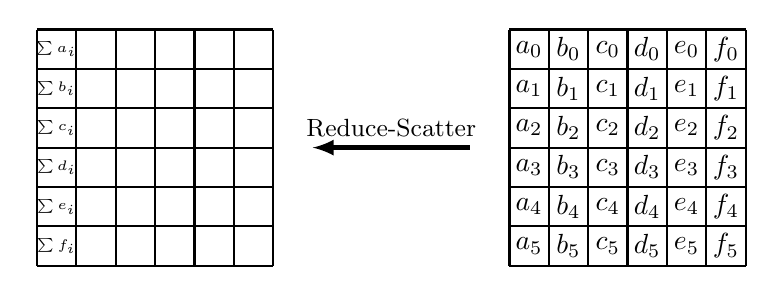
\begin{tikzpicture}[scale=0.5, >=latex]
%Bcast
\begin{scope}
  \begin{scope}
    \foreach \i in {0,1,...,6} {
      \draw[thick] (\i, 0) -- +(0, 6);
      \draw[thick] (0, \i) -- +(6, 0);
    }
    
    \node at (0.5, 5.5) {$\scriptscriptstyle \sum a_i$};
    \node at (0.5, 4.5) {$\scriptscriptstyle \sum b_i$};
    \node at (0.5, 3.5) {$\scriptscriptstyle \sum c_i$};
    \node at (0.5, 2.5) {$\scriptscriptstyle \sum d_i$};
    \node at (0.5, 1.5) {$\scriptscriptstyle \sum e_i$};
    \node at (0.5, 0.5) {$\scriptscriptstyle \sum f_i$};
  \end{scope}

\draw[ultra thick,<-] (7, 3) -- node[above,font=\small] {Reduce-Scatter} (11, 3);

\begin{scope}[xshift=12cm]
  \foreach \i in {0,1,...,6} {
    \draw[thick] (\i, 0) -- +(0, 6);
    \draw[thick] (0, \i) -- +(6, 0);
  }
  \foreach \i in {0,1,...,5} {
    \node at (0.5, 5.5-\i) {$a_\i$};
    \node at (1.5, 5.5-\i) {$b_\i$};
    \node at (2.5, 5.5-\i) {$c_\i$};
    \node at (3.5, 5.5-\i) {$d_\i$};
    \node at (4.5, 5.5-\i) {$e_\i$};
    \node at (5.5, 5.5-\i) {$f_\i$};
  }
\end{scope}
\end{scope}
\end{tikzpicture}
\end{center}

\begin{itemize}
\item Lower bound: $T \geq \lceil \log_2 p \rceil \alpha + (p-1) \frac{n}{p} \beta$
\item Ring algorithm: $T = (p-1) (\alpha + \frac{n}{p} \beta)$
\end{itemize}

\end{frame}



%%%%%%%%%%%%%%%%%%%%%%%%%%%%%%%%%%%%%%%%%%%%

\begin{frame}[label=2d]
  \frametitle{Distributed Matrix-Vector Product}
  \framesubtitle{2D block distribution}

  \begin{block}{Data distribution}
    \begin{itemize}
    \item[$M$] : 2D block distribution ($v \times h$ blocks)
    \item[$x$] : 1D block distribution 
    \item[$y$] : 1D block distribution
    \end{itemize}
  \end{block}

  \begin{center}
    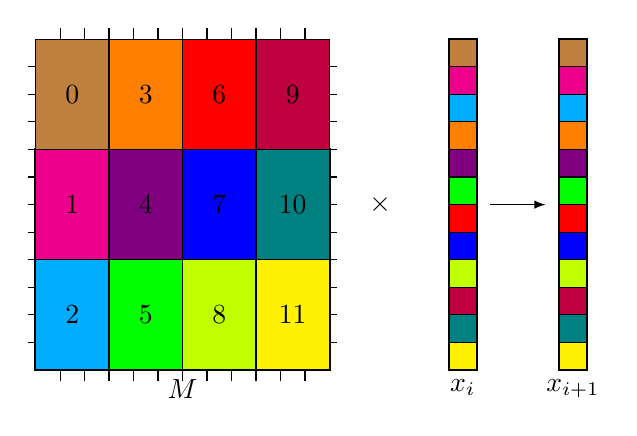
\begin{tikzpicture}[>=latex, scale=0.7]
      \begin{scope}[xshift=-4cm, yscale=2, xscale=1.333]
        \draw[thick] (0,0) rectangle (4,2);
        \foreach \i in {1, 2, ..., 11} {
          \draw (-0.1, \i/4) -- (0, \i/4);
          \draw (\i/3, -0.1) -- (\i/3, 0);
          \draw (4.1, \i/4) -- (4, \i/4);
          \draw (\i/3, 3.1) -- (\i/3, 3);
        }
      \filldraw[fill=brown]    (0, 2) rectangle node {0} +(1, 1);
      \filldraw[fill=orange]   (1, 2) rectangle  node {3} +(1, 1);
      \filldraw[fill=red]      (2, 2) rectangle  node {6} +(1, 1);
      \filldraw[fill=purple]   (3, 2) rectangle  node {9} +(1, 1);
      \filldraw[fill=magenta]  (0, 1) rectangle  node {1} +(1, 1);
      \filldraw[fill=violet]   (1, 1) rectangle  node {4} +(1, 1);
      \filldraw[fill=blue]     (2, 1) rectangle  node {7} +(1, 1);
      \filldraw[fill=teal]     (3, 1) rectangle  node {10} +(1, 1);
      \filldraw[fill=cyan]     (0, 0) rectangle  node {2} +(1, 1);
      \filldraw[fill=green]    (1, 0) rectangle  node {5} +(1, 1);
      \filldraw[fill=lime]     (2, 0) rectangle  node {8} +(1, 1);
      \filldraw[fill=yellow]   (3, 0) rectangle  node {11} +(1, 1);

      \node[below] at (2,0) {$M$};
    \end{scope}

    \node at (2.25, 3) {$\times$};

          \begin{scope}[xshift=-1cm]
      \draw[thick] (4.5,0) rectangle +(0.5, 6);
      \filldraw[fill=brown]    (4.5, 5.5) rectangle   +(0.5, 0.5);
      \filldraw[fill=magenta]   (4.5, 5) rectangle     +(0.5, 0.5);
      \filldraw[fill=cyan]     (4.5, 4.5) rectangle   +(0.5, 0.5);
      \filldraw[fill=orange]    (4.5, 4) rectangle     +(0.5, 0.5);
      \filldraw[fill=violet]  (4.5, 3.5) rectangle   +(0.5, 0.5);
      \filldraw[fill=green]   (4.5, 3) rectangle     +(0.5, 0.5);
      \filldraw[fill=red]     (4.5, 2.5) rectangle   +(0.5, 0.5);
      \filldraw[fill=blue]     (4.5, 2) rectangle     +(0.5, 0.5);
      \filldraw[fill=lime]      (4.5, 1.5) rectangle   +(0.5, 0.5);
      \filldraw[fill=purple]    (4.5, 1) rectangle     +(0.5, 0.5);
      \filldraw[fill=teal]     (4.5, 0.5) rectangle   +(0.5, 0.5);
      \filldraw[fill=yellow]   (4.5, 0) rectangle     +(0.5, 0.5);
      \node[below] at (4.75,0) {$x_i$};
    \end{scope}
    \draw[->] (4.25, 3) -- +(1,0);
      
      \begin{scope}[xshift=1cm]
              \draw[thick] (4.5,0) rectangle +(0.5, 6);
      \filldraw[fill=brown]    (4.5, 5.5) rectangle   +(0.5, 0.5);
      \filldraw[fill=magenta]   (4.5, 5) rectangle     +(0.5, 0.5);
      \filldraw[fill=cyan]     (4.5, 4.5) rectangle   +(0.5, 0.5);
      \filldraw[fill=orange]    (4.5, 4) rectangle     +(0.5, 0.5);
      \filldraw[fill=violet]  (4.5, 3.5) rectangle   +(0.5, 0.5);
      \filldraw[fill=green]   (4.5, 3) rectangle     +(0.5, 0.5);
      \filldraw[fill=red]     (4.5, 2.5) rectangle   +(0.5, 0.5);
      \filldraw[fill=blue]     (4.5, 2) rectangle     +(0.5, 0.5);
      \filldraw[fill=lime]      (4.5, 1.5) rectangle   +(0.5, 0.5);
      \filldraw[fill=purple]    (4.5, 1) rectangle     +(0.5, 0.5);
      \filldraw[fill=teal]     (4.5, 0.5) rectangle   +(0.5, 0.5);
      \filldraw[fill=yellow]   (4.5, 0) rectangle     +(0.5, 0.5);
      \node[below] at (4.75,0) {$x_{i+1}$};
    \end{scope}

  \end{tikzpicture}
\end{center}
\end{frame}

%%%%%%%%%%%%%%%%%%%%%%%%%%%%%%%%%%%

\begin{frame}[label=2d]
  \begin{columns}
    \begin{column}{6cm}
    \begin{tikzpicture}[>=latex,scale=0.4]
      \begin{scope}[xshift=-4cm, yscale=2, xscale=1.5]
        \foreach \i in {1, 2, ..., 11} {
          \draw (-0.1, \i/4) -- (0, \i/4);
          \draw (\i/3, -0.1) -- (\i/3, 0);
          \draw (4.1, \i/4) -- (4, \i/4);
          \draw (\i/3, 3.1) -- (\i/3, 3);
        }
      \filldraw[fill=brown]    (0, 2) rectangle node {0} +(1, 1);
      \filldraw[fill=orange]   (1, 2) rectangle  node {3} +(1, 1);
      \filldraw[fill=red]      (2, 2) rectangle  node {6} +(1, 1);
      \filldraw[fill=purple]   (3, 2) rectangle  node {9} +(1, 1);
      \filldraw[fill=magenta]  (0, 1) rectangle  node {1} +(1, 1);
      \filldraw[fill=violet]   (1, 1) rectangle  node {4} +(1, 1);
      \filldraw[fill=blue]     (2, 1) rectangle  node {7} +(1, 1);
      \filldraw[fill=teal]     (3, 1) rectangle  node {10} +(1, 1);
      \filldraw[fill=cyan]     (0, 0) rectangle  node {2} +(1, 1);
      \filldraw[fill=green]    (1, 0) rectangle  node {5} +(1, 1);
      \filldraw[fill=lime]     (2, 0) rectangle  node {8} +(1, 1);
      \filldraw[fill=yellow]   (3, 0) rectangle  node {11} +(1, 1);
      \draw[thick] (0,0) rectangle (4, 3);
      
      \draw<2>[pattern=north east lines] (0, 2) rectangle  +(1/3, 1);
      \draw<2>[pattern=north east lines] (1, 2) rectangle  +(1/3, 1);
      \draw<2>[pattern=north east lines] (2, 2) rectangle  +(1/3, 1);
      \draw<2>[pattern=north east lines] (3,   2) rectangle  +(1/3, 1);
      \draw<2>[pattern=north east lines] (1/3, 1) rectangle  +(1/3, 1);
      \draw<2>[pattern=north east lines] (1+1/3, 1) rectangle  +(1/3, 1);
      \draw<2>[pattern=north east lines] (2+1/3, 1) rectangle  +(1/3, 1);
      \draw<2>[pattern=north east lines] (3+1/3, 1) rectangle  +(1/3, 1);
      \draw<2>[pattern=north east lines] (0+2/3, 0) rectangle  +(1/3, 1);
      \draw<2>[pattern=north east lines] (1+2/3, 0) rectangle  +(1/3, 1);
      \draw<2>[pattern=north east lines] (2+2/3, 0) rectangle  +(1/3, 1);
      \draw<2>[pattern=north east lines] (3+2/3, 0) rectangle  +(1/3, 1);

      \node[below] at (2,0) {$M$};
    \end{scope}

    \begin{onlyenv}<9-10>
      \begin{scope}[xshift=4cm, yscale=2, xscale=1.5]
        \foreach \i in {1, 2, ..., 11} {
          \draw (-0.1, \i/4) -- (0, \i/4);
          \draw (\i/3, -0.1) -- (\i/3, 0);
          \draw (4.1, \i/4) -- (4, \i/4);
          \draw (\i/3, 3.1) -- (\i/3, 3);
        }
      \filldraw[fill=brown]    (0, 2) rectangle node {0} +(1, 1);
      \filldraw[fill=magenta]  (1, 2) rectangle  node {1} +(1, 1);
      \filldraw[fill=cyan]     (2, 2) rectangle  node {2} +(1, 1);      
      \filldraw[fill=orange]   (3, 2) rectangle  node {3} +(1, 1);
      
      \filldraw[fill=violet]   (0, 1) rectangle  node {4} +(1, 1);
      \filldraw[fill=green]    (1, 1) rectangle  node {5} +(1, 1);
      \filldraw[fill=red]      (2, 1) rectangle  node {6} +(1, 1);
      \filldraw[fill=blue]     (3, 1) rectangle  node {7} +(1, 1);
      
      \filldraw[fill=lime]     (0, 0) rectangle  node {8} +(1, 1);
      \filldraw[fill=purple]   (1, 0) rectangle  node {9} +(1, 1);
      \filldraw[fill=teal]     (2, 0) rectangle  node {10} +(1, 1);
      \filldraw[fill=yellow]   (3, 0) rectangle  node {11} +(1, 1);
      \draw[thick] (0,0) rectangle (4, 3);
    \end{scope}
  \end{onlyenv}
\end{tikzpicture}

    \begin{block}{Algorithm}
      \begin{itemize}
      \item<3-> \texttt{MPI\_Allgather}
      \item<5-> \texttt{GEMV} (partial sums)
      \item<7-> \texttt{MPI\_reduce\_scatter}
      \item<10-> \texttt{MPI\_sendrecv} (transpose)

      \end{itemize}
    \end{block}
  \end{column}

  \begin{column}{4cm}
    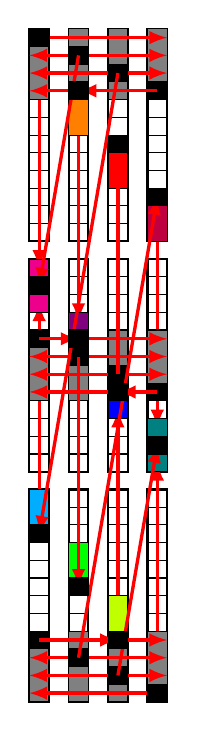
\begin{tikzpicture}[>=latex, yscale=0.45, xscale=0.5]
      % cadre
      \foreach \i in {0, 1, 2, 3} {
        \foreach \j in {0, 1, 2} {
          \draw[thick] (\i, 6.5*\j) rectangle +(0.5, 6);
          \foreach \k in {1, 2, ..., 11} {
            \draw (\i, 6.5*\j) ++(0, 0.5*\k) -- ++(0.5, 0);
          }
        }
      }

      % placement initial
      \foreach \i in {0, 1, 2, 3} {
        \foreach \j in {0, 1, 2} {
          \filldraw<1-3>[fill=black]  (\i, 3*6 + 0.5 - 1.5*\i - 7*\j)  rectangle +(0.5, 0.5);
        }
      }

      % Allgather colonnes arrows
      \draw<3>[red, very thick, <->] (0.25, 5.25 + 2*6.5) -- +(0, -6);
      \draw<3>[red, very thick, <->] (0.25, 4.75 + 1*6.5) -- +(0, -6);
      \draw<3>[red, very thick, <->] (1.25, 3.75 + 2*6.5) -- +(0, -6);
      \draw<3>[red, very thick, <->] (1.25, 3.25 + 1*6.5) -- +(0, -6);
      \draw<3>[red, very thick, <->] (2.25, 2.25 + 2*6.5) -- +(0, -6);
      \draw<3>[red, very thick, <->] (2.25, 1.75 + 1*6.5) -- +(0, -6);
      \draw<3>[red, very thick, <->] (3.25, 0.75 + 2*6.5) -- +(0, -6);
      \draw<3>[red, very thick, <->] (3.25, 0.25 + 1*6.5) -- +(0, -6);

      % allgather result
      \foreach \i in {0, 1, 2, 3} {
        \foreach \j in {0, 1, 2} {
          \filldraw<4>[fill=black]  (\i, 3*6 - 0.5 - 1.5*\i - 6.5*\j)  rectangle +(0.5, 1.5);
        }
      }

      % prepare GEMM
      \filldraw<5>[fill=brown]       (0, 17.5)   rectangle +(0.5, 1.5);
      \filldraw<5>[fill=orange]      (1, 16) rectangle +(0.5, 1.5);
      \filldraw<5>[fill=red]         (2, 14.5)   rectangle +(0.5, 1.5);
      \filldraw<5>[fill=purple]      (3, 13)   rectangle +(0.5, 1.5);
      \filldraw<5>[fill=magenta]     (0, 11)    rectangle +(0.5, 1.5);
      \filldraw<5>[fill=violet]      (1, 9.5)  rectangle +(0.5, 1.5);
      \filldraw<5>[fill=blue]        (2, 8)    rectangle +(0.5, 1.5);
      \filldraw<5>[fill=teal]        (3, 6.5)    rectangle +(0.5, 1.5);
      \filldraw<5>[fill=cyan]        (0, 4.5)    rectangle +(0.5, 1.5);
      \filldraw<5>[fill=green]       (1, 3)  rectangle +(0.5, 1.5);
      \filldraw<5>[fill=lime]        (2, 1.5)    rectangle +(0.5, 1.5);
      \filldraw<5>[fill=yellow]      (3, 0)    rectangle +(0.5, 1.5);


      % GEMM result
      \foreach \i in {0, 1, 2, 3} {
        \foreach \j in {0, 1, 2} {
          \filldraw<6-7>[fill=gray]  (\i, 2*\j + 6.5*\j)  rectangle +(0.5, 2);
        }
      }

      % Reduce-scatter arrow
      \foreach \i in {0, 1, 2, 3} {
        \foreach \j in {0, 1, 2} {
          \draw<7>[red,very thick, <->]  (0, 0.25 + 8.5*\j + 0.5*\i) -- +(3.5, 0);
        }
      }

      % placement après RS
      \foreach \i in {0, 1, 2, 3} {
        \foreach \j in {0, 1, 2} {
          \filldraw<8-10>[fill=black]  (\i, 1.5 - 0.5*\i +2*\j + 6.5*\j)  rectangle +(0.5, 0.5);
        }
      }

      % transposition
      \draw<10>[red, very thick,->]  (1.25, 5.25 + 2*6.5)  --  (0.25, 5.25 + 1*6.5);
      \draw<10>[red, very thick,->]  (2.25, 4.75 + 2*6.5)  --  (0.25, 4.75 + 0*6.5);
      \draw<10>[red, very thick,->]  (3.25, 4.25 + 2*6.5)  --  (1.25, 4.25 + 2*6.5);
      \draw<10>[red, very thick,->]  (0.25, 3.75 + 1*6.5)  --  (1.25, 3.75 + 1*6.5);
      \draw<10>[red, very thick,->]  (1.25, 3.25 + 1*6.5)  --  (1.25, 3.25 + 0*6.5);
      \draw<10>[red, very thick,->]  (2.25, 2.75 + 1*6.5)  --  (2.25, 2.75 + 2*6.5);
      \draw<10>[red, very thick,->]  (3.25, 2.25 + 1*6.5)  --  (2.25, 2.25 + 1*6.5);
      \draw<10>[red, very thick,->]  (0.25, 1.75 + 0*6.5)  --  (2.25, 1.75 + 0*6.5);
      \draw<10>[red, very thick,->]  (1.25, 1.25 + 0*6.5)  --  (3.25, 1.25 + 2*6.5);
      \draw<10>[red, very thick,->]  (2.25, 0.75 + 0*6.5)  --  (3.25, 0.75 + 1*6.5);

      % retour au placement initial
      \foreach \i in {0, 1, 2, 3} {
        \foreach \j in {0, 1, 2} {
          \filldraw<11>[fill=black]  (\i, 3*6 + 0.5 - 1.5*\i - 7*\j)  rectangle +(0.5, 0.5);
        }
      }
    \end{tikzpicture}
  \end{column}
\end{columns}
\end{frame}

%%%%%%%%%%%%%%%%%%%%%%%%%%%%%%%

\begin{frame}[fragile,label=2d]
\frametitle{MPI: sub-communicators}

\begin{minted}[fontsize=\scriptsize]{C}
int MPI_Comm_split(MPI_Comm comm, int color, int key, MPI_Comm *newcomm);
\end{minted}

\medskip

\begin{itemize}
\item \textbf{Collective} operation (all processess in \texttt{comm} call it)
\item \red{Partitions} \texttt{comm} into sub-communicators according to \texttt{color} 
  \begin{itemize}
  \item $P_i$ and $P_j$ give color $k$ $\leadsto$ belong to the same \texttt{newcomm}
  \end{itemize}
\item Within \texttt{newcomm}, processes ranked by increasing \texttt{key}
  \begin{itemize}
  \item \texttt{key} need not be consecutive; MPI does the (distributed) sort
    
  \end{itemize}
\end{itemize}

\begin{block}{Example: Rows and Columns}
  \begin{minted}[fontsize=\scriptsize]{C}
    // matrix distributed into a v * h process grid
    // split MPI_COMM_WORLD into v row communicators
    //                           h column communicators
    int i = rank % v;
    int j = rank / v;
    // I have the (i, j) matrix sub-block
    MPI_Comm_split(MPI_COMM_WORLD, i, j, &row_comm);
    MPI_Comm_split(MPI_COMM_WORLD, j, i, &col_comm);
  \end{minted}
\end{block}

\end{frame}


%%%%%%%%%%%%%%%%%%%%%%%%%%%%%%%%

\begin{frame}[label=2d]
  \frametitle{Analysis}

  Process grid of size $v \times h$
  
  \begin{center}
    \begin{tabular}{|c||c|c|}
      \hline
      & Sequential & Distributed \\
      \hline\hline
      \texttt{GEMV}                 & $3 d n^2 / C$ & $3 d n^2 / (vhC)$ \\
      \hline
      \texttt{MPI\_Allgather}       & 0             & $n / (hD)$ \\
      \hline
      \texttt{MPI\_reduce\_scatter} & 0             & $n / (vD)$ \\
      \hline
      \texttt{MPI\_sendrecv}        & 0             & $n / (vhD)$ \\
      \hline
    \end{tabular}
  \end{center}

  Assume $v = h = \sqrt{p}$.
  
  \[
    \mathrm{Speedup} = \frac{d n^2}{C} / (\frac{d n^2}{pC} + \frac{n}{D\sqrt{p}})
  \]

  \begin{alertblock}{Progress}
    \begin{itemize}
    \item Communication time \textbf{also decreases} when $p$ grows
    \item Speed-up \textbf{no longer bounded} when $p$ grows
    \end{itemize}
  \end{alertblock}
  
\end{frame}


\end{document}

%%% Local Variables:
%%% TeX-command-extra-options: "-shell-escape"
%%% TeX-engine: xetex
%%% End: